\documentclass[tikz,border=7pt]{standalone}
\usepackage{amsmath,amssymb}
\usetikzlibrary{arrows.meta,calc,positioning,decorations.pathreplacing}

\newcommand{\R}{\mathbb{R}}

% ============================================================
% FOUR explicit, sphere-specialized figures at p = (0,0,1):
%   (1) Gauss map  N:S^2->S^2,  p |-> p (outward normal)
%   (2) Differential (dN)_p computed from a concrete curve gamma(t)
%   (3) Identification of planes:  T_pS^2 = (N(p))^\perp = T_{N(p)}S^2  inside R^3
%   (4) Shape operator S_p = -(dN)_p and its diagonal matrix in a chosen basis
%
% For clarity, (1),(2),(4) use the xz cross-section (y=0) where S^2 is the unit circle.
% Figure (3) uses a clean 3D-style schematic: the plane z=1 through p.
% ============================================================

\begin{document}	
% ============================================================
% (1) Gauss map N: S^2 -> S^2, N(p)=p  (identity map)
% ============================================================	
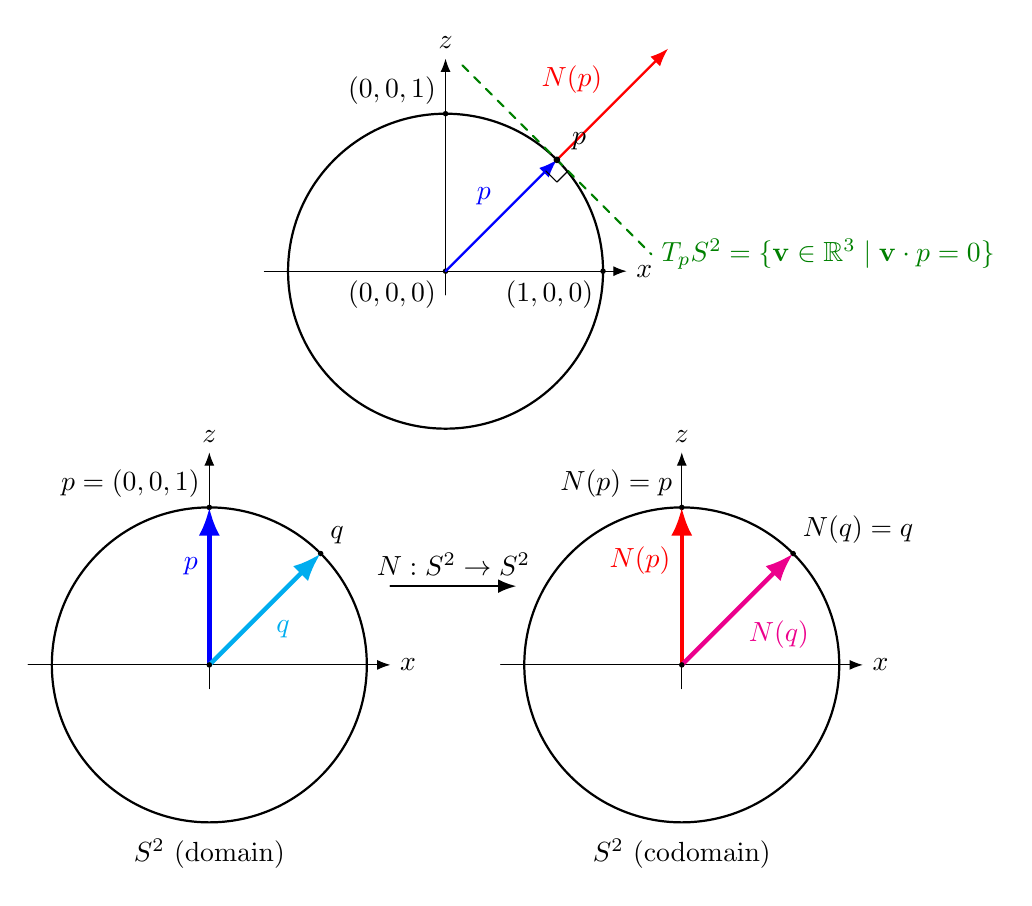
\begin{tikzpicture}[>=Latex, line cap=round, line join=round, scale=2]
	\begin{scope}[shift={(1.5,2.5)}]
	\def\angle{45} 
	\def\d{0.1} % Size of the right-angle square
	\coordinate (O) at (0,0);
	\coordinate (P) at ({\angle}:1); 
		
	\draw[thick] (0,0) circle (1);
	\fill[thick] (0,0) circle (.5pt);
	\draw[->] (-1.15,0) -- (1.15,0) node[right] {$x$};
	\draw[->] (0,-0.15) -- (0,1.35) node[above] {$z$};
	\node[anchor=north east] at (0,0) {$(0,0,0)$};
	\fill[thick] (0,1) circle (.5pt);
	\node[anchor=south east] at (0,1) {$(0,0,1)$};
	\fill[thick] (1,0) circle (.5pt);
	\node[anchor=north east] at (1,0) {$(1,0,0)$};
	
	% 5. The Normal Vector N(p)
	\draw[red, thick, ->] (P) -- ++(0.707, 0.707) node[midway, above left] {$N(p)$};

	% --- 2. RADIUS & NORMAL ---
	\draw[blue, thick, ->] (O) -- (P) node[midway, above left, color=blue] {$p$};
	
	% --- 3. THE TANGENT SPACE ---
	\draw[green!50!black, thick, dashed] 
	($(P) + (-0.6, 0.6)$) -- 
	($(P) + (0.6, -0.6)$) node[right] {
		$T_p S^2 = \{ \mathbf{v} \in \mathbb{R}^3 \mid \mathbf{v} \cdot p = 0 \}$
	};
	
	% --- 4. CORRECT SQUARE MARKER ---
	\coordinate (R) at ($(P)!\d!(O)$);
	\coordinate (T) at ($(P)!\d!90:(O)$);
	\coordinate (Corner) at ($(R) + (T) - (P)$);
	% Draw the square path
	\draw[black, thin] (R) -- (Corner) -- (T);
	% Point P
	\filldraw (P) circle (0.5pt) node[anchor=south west, xshift=2pt] {$p$};
	\end{scope}
	
	\begin{scope}[shift={(0,0)}]
		\draw[thick] (0,0) circle (1);
		\node at (0,-1.2) {$S^2$ (domain)};
		\draw[->] (-1.15,0) -- (1.15,0) node[right] {$x$};
		\draw[->] (0,-0.15) -- (0,1.35) node[above] {$z$};
		
		\coordinate (pL) at (0,1);
		\fill (pL) circle (0.5pt) node[above left] {$p=(0,0,1)$};
		\fill (.707,.707) circle (0.5pt) node[above right] {$q$};
		
		\draw[blue, ultra thick, ->] (0,0) -- (0,1) node[midway, above left, color=blue] {$p$};
		\draw[cyan, ultra thick, ->] (0,0) -- (.707,.707) node[midway, below right] {$q$};
		\fill[thick] (0,0) circle (.5pt);
	\end{scope}
	
	\begin{scope}[shift={(3,0)}]
		\draw[thick] (0,0) circle (1);
		\node at (0,-1.2) {$S^2$ (codomain)};
		\draw[->] (-1.15,0) -- (1.15,0) node[right] {$x$};
		\draw[->] (0,-0.15) -- (0,1.35) node[above] {$z$};
		
		\coordinate (pR) at (0,1);
		\fill (pR) circle (0.5pt) node[above left] {$N(p)=p$};
		\fill (.707,.707) circle (0.5pt) node[above right] {$N(q)=q$};
		\draw[red, ultra thick, ->] (0,0) -- (0,1) node[midway, above left, color=red] {$N(p)$};
		\draw[magenta, ultra thick, ->] (0,0) -- (.707,.707) node[midway, below right] {$N(q)$};
		\fill[thick] (0,0) circle (.5pt);
	\end{scope}
	
	\draw[thick,->] (1.15,.5) -- (1.95,.5) node[midway, above] {$N:S^2\to S^2$};
		
\end{tikzpicture}
\end{document}